\documentclass[11pt]{article}

\usepackage[margin=1in]{geometry}
\usepackage{graphicx}
\usepackage{setspace}
\usepackage{caption}
\usepackage{float}
\usepackage{url}

\onehalfspacing

\title{\textbf{Supplement S2: Additional Figures}\\[0.5cm]
\large Outbreak Forecasting, Methamphetamine Trajectories, Scenario Comparisons, Cascade Uncertainty, R\_0ZeroDistributions, Barrier Removal Impact and Step Importance\\[0.5cm]
\normalsize Supporting the manuscript:\\
\textbf{Structural barriers drive near-zero population-level effectiveness of Long Acting Injectable HIV prevention (LAI-PrEP) among people who inject drugs:}\\
\textbf{A Computational Modeling Study}}

\author{AC Demidont, DO\\Independent Researcher, Nyx Dynamics LLC}
\date{December 27, 2025}

\begin{document}

\maketitle


\section*{Supplementary Figures}

\begin{figure}[H]
\centering
\includegraphics[width=\textwidth]{FigS1_MethTrajectories.png}
\caption*{Figure S1}
\end{figure}

\begin{figure}[H]
\centering
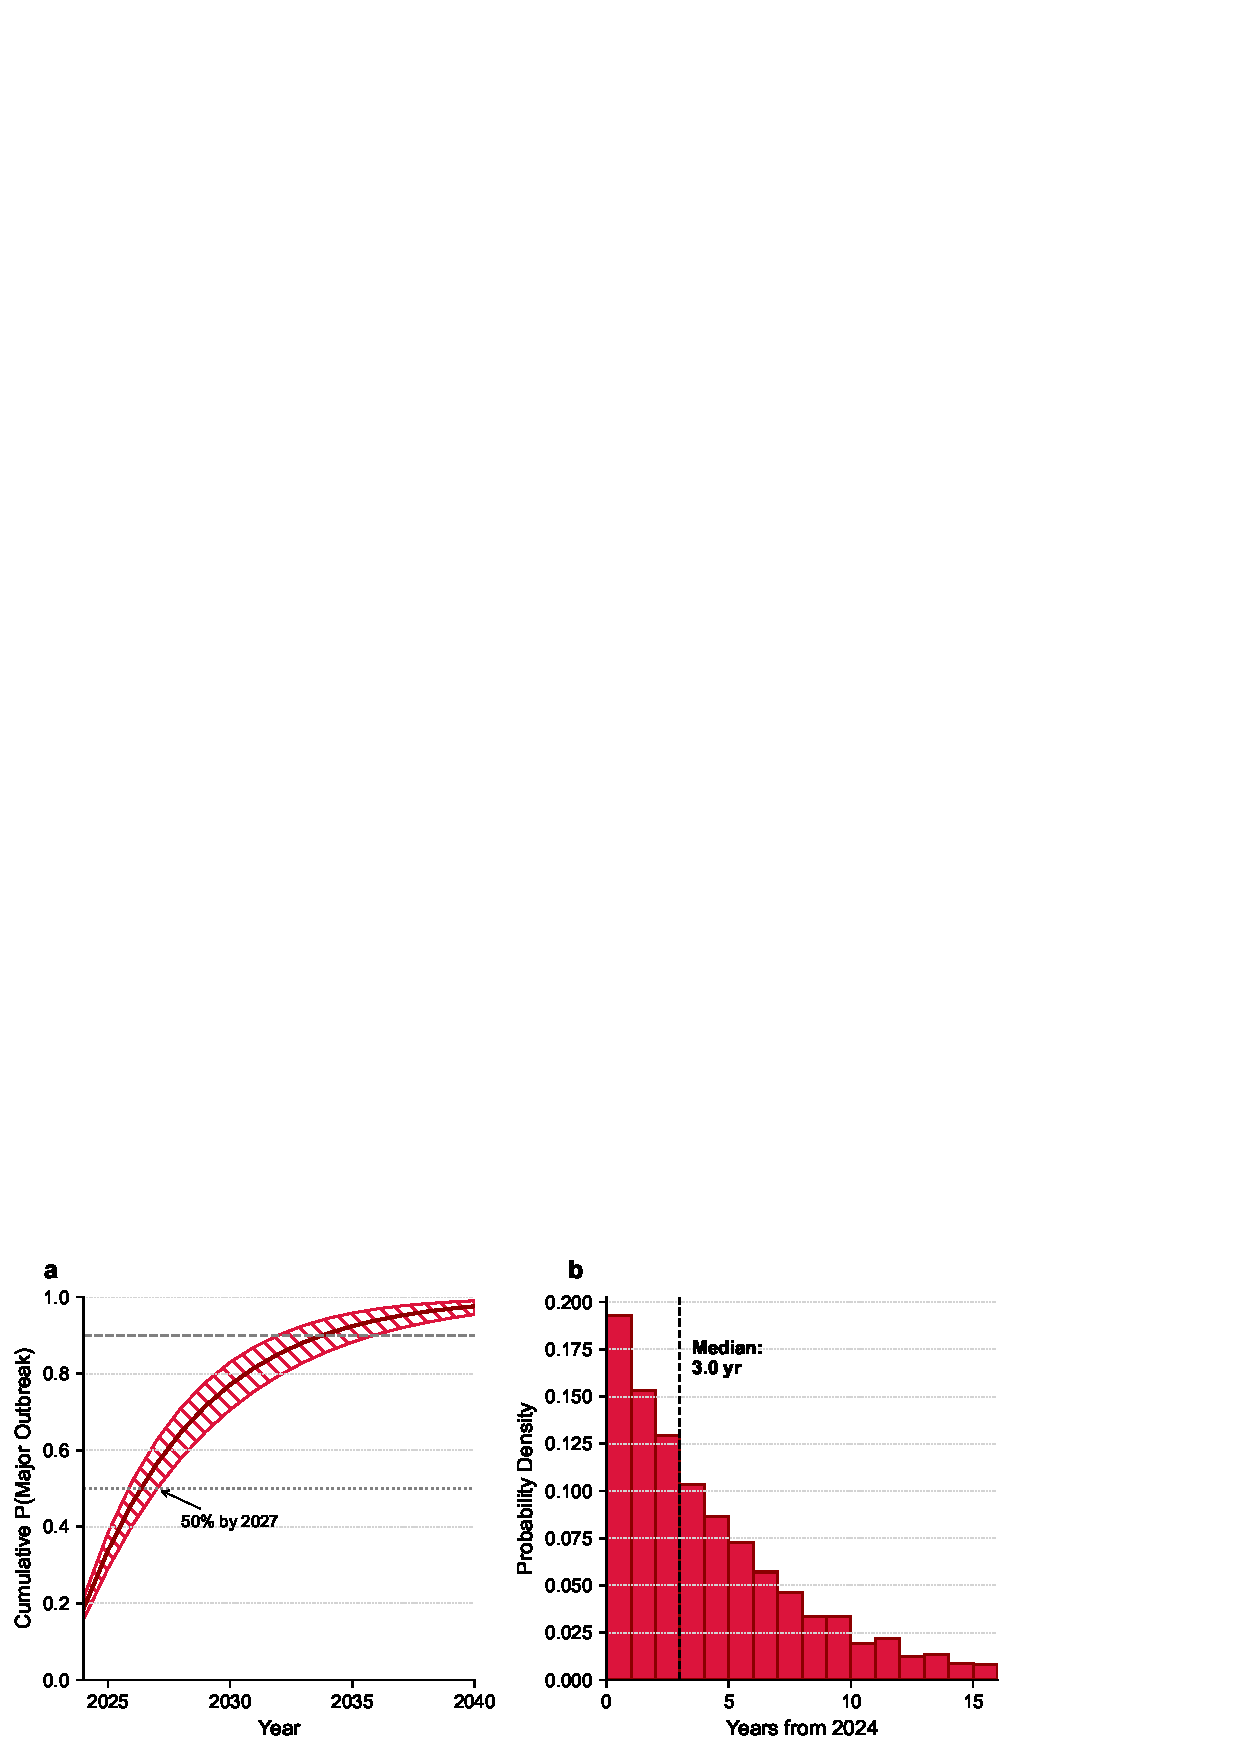
\includegraphics[width=\textwidth]{FigS2_OutbreakForecast.png}
\caption*{Figure S2}
\end{figure}

\begin{figure}[H]
\centering
\includegraphics[width=\textwidth]{FigS3_TornadoDiagram.png}
\caption*{Figure S3}
\end{figure}

\begin{figure}[H]
\centering
\includegraphics[width=\textwidth]{FigS4_ScenarioComparison.png}
\caption*{Figure S4}
\end{figure}

\begin{figure}[H]
\centering
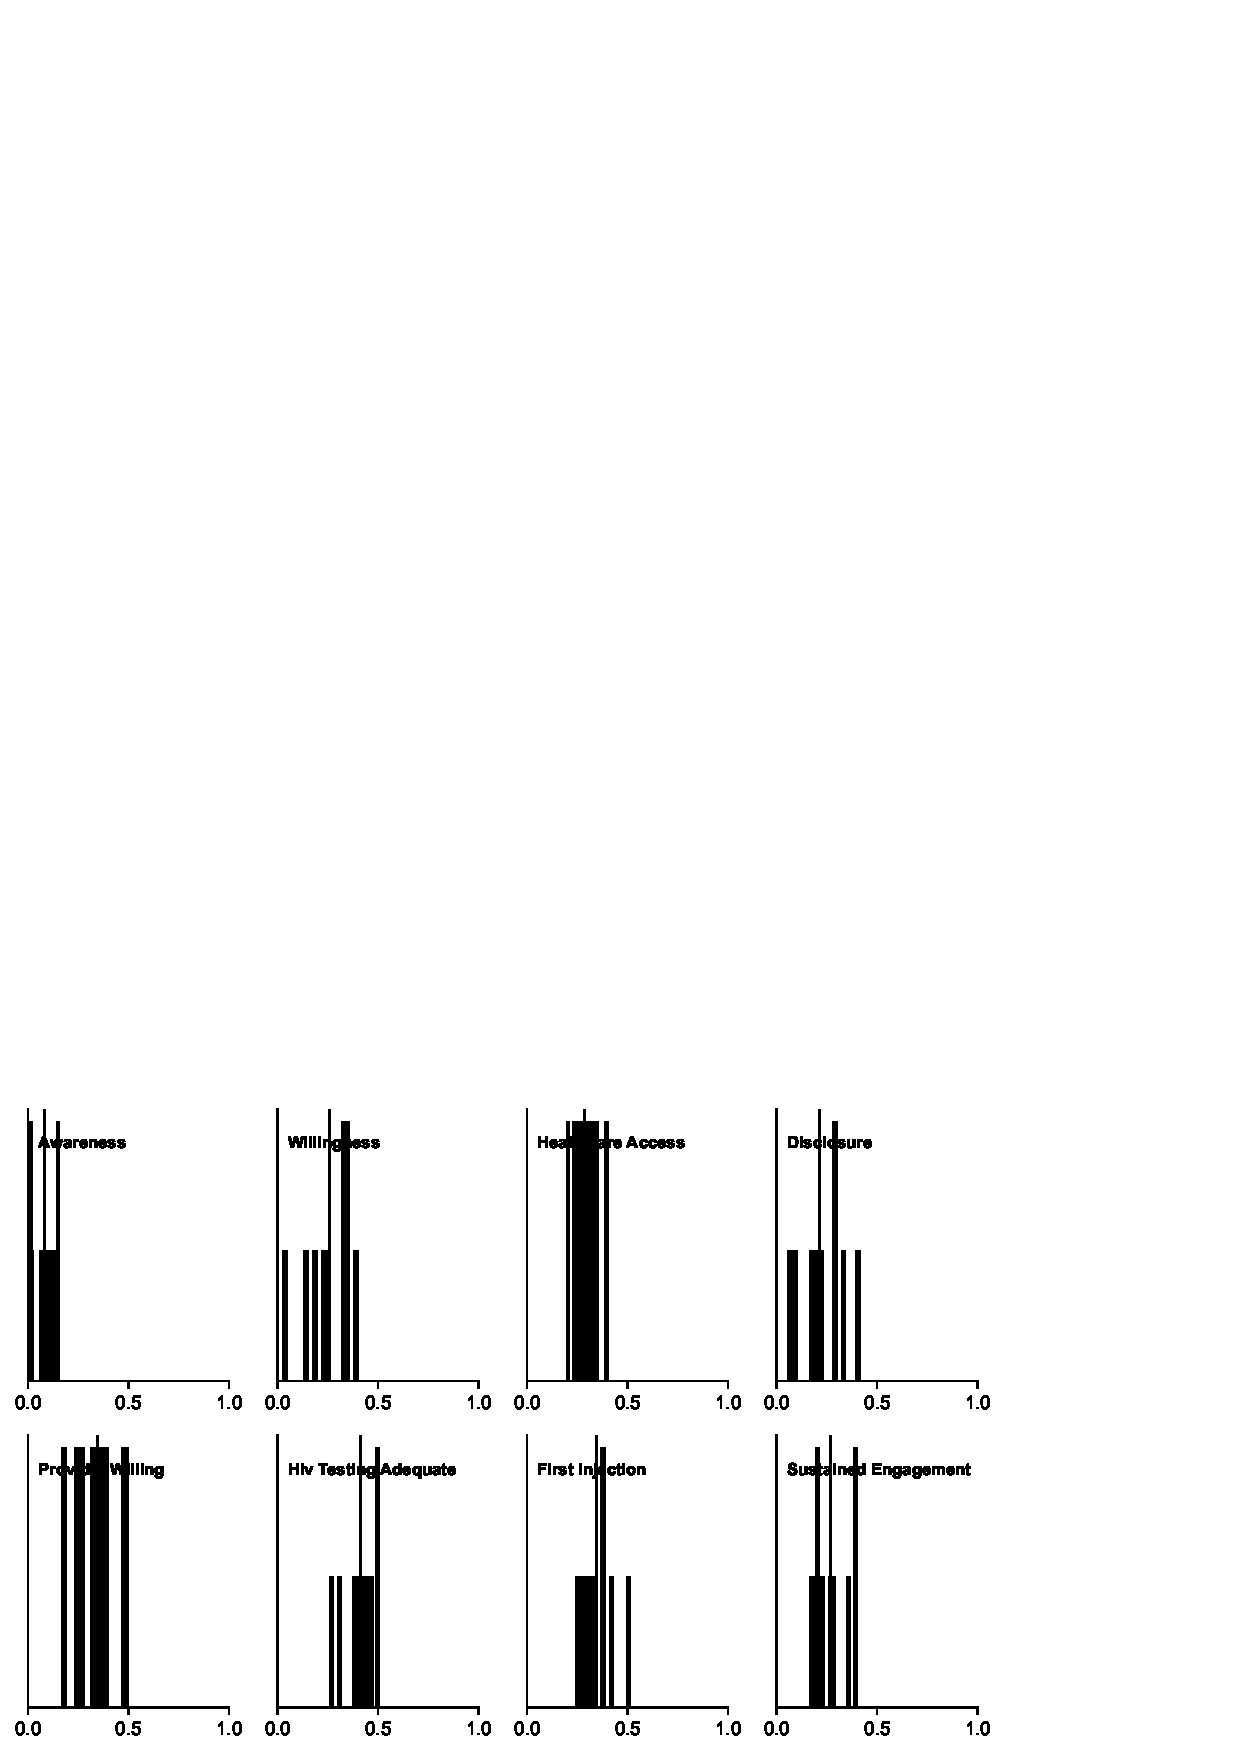
\includegraphics[width=\textwidth]{FigS5_CascadeUncertainty.png}
\caption*{Figure S5}
\end{figure}

\begin{figure}[H]
\centering
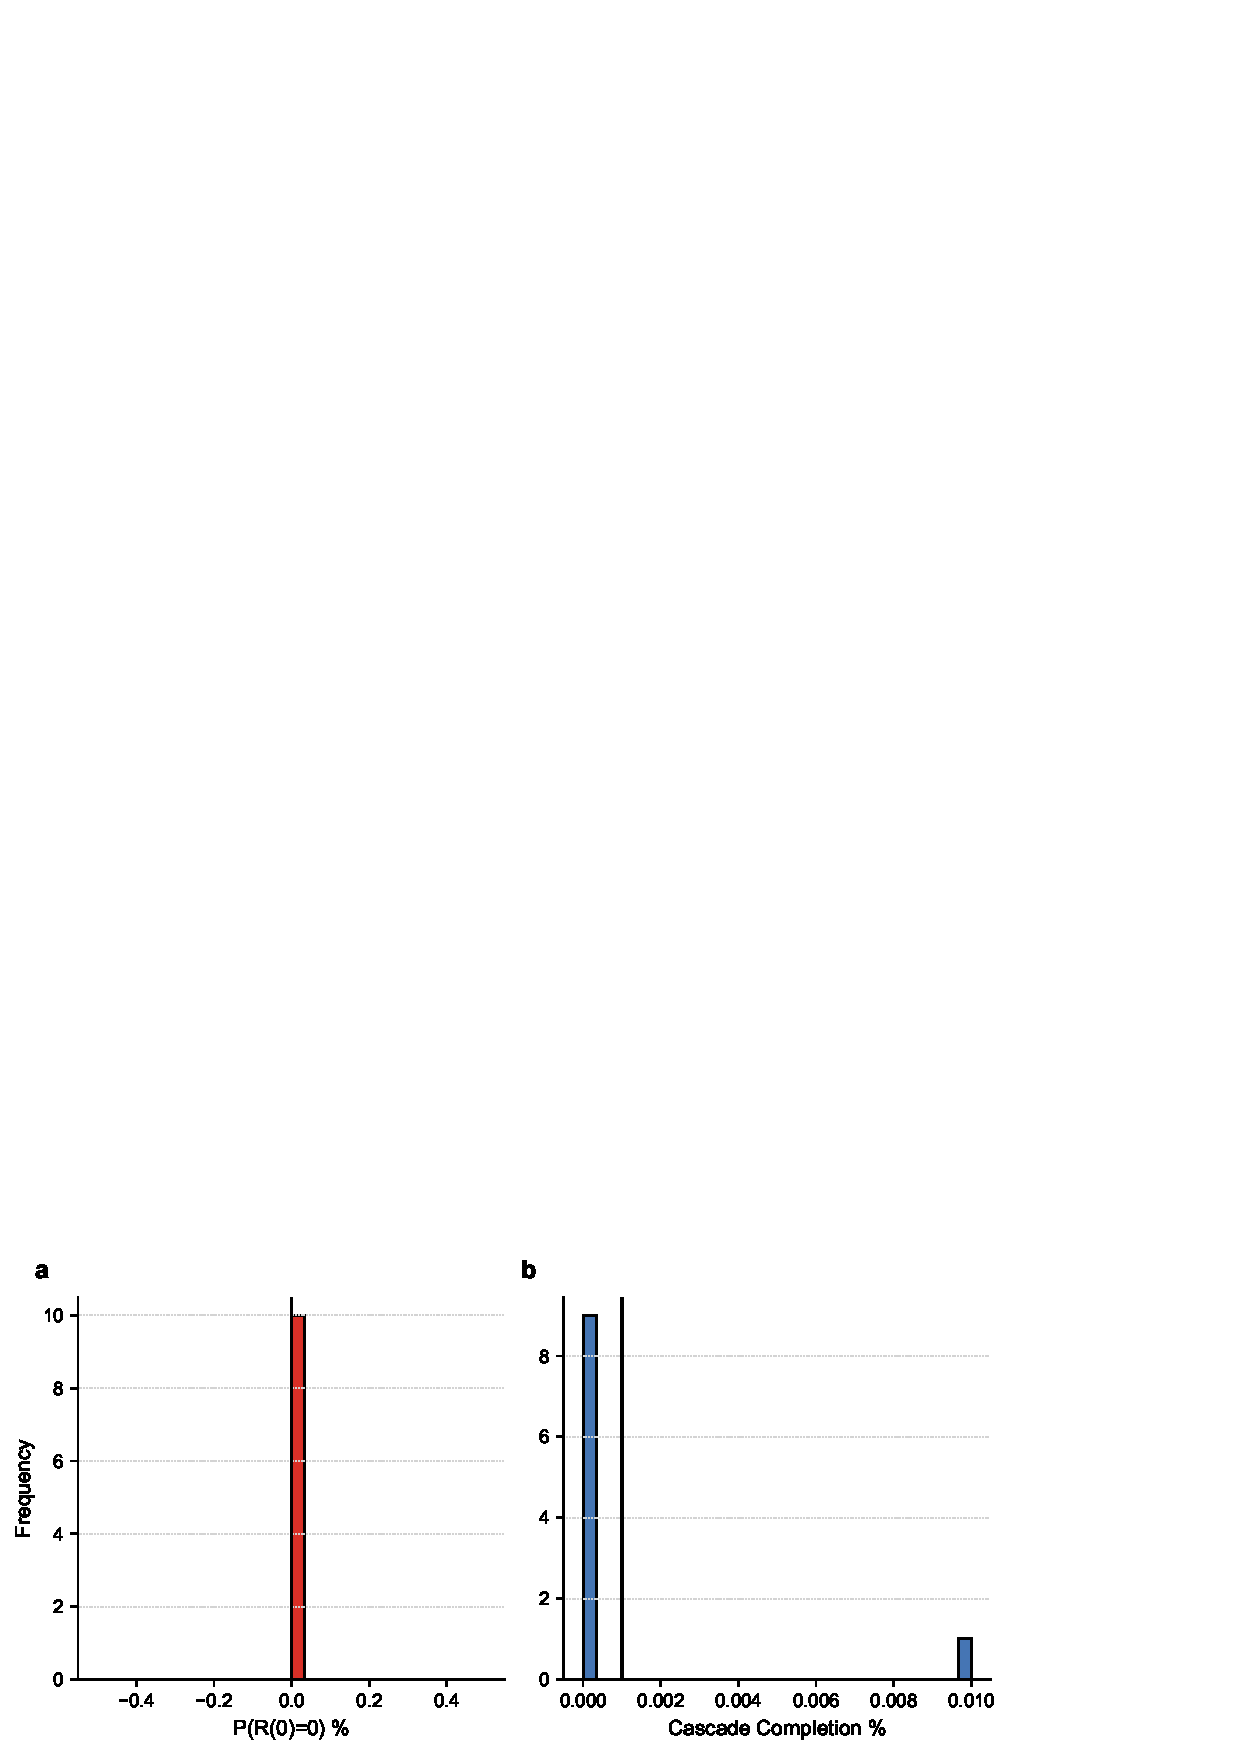
\includegraphics[width=\textwidth]{FigS6_R0ZeroDistribution.png}
\caption*{Figure S6}
\end{figure}

\begin{figure}[H]
\centering
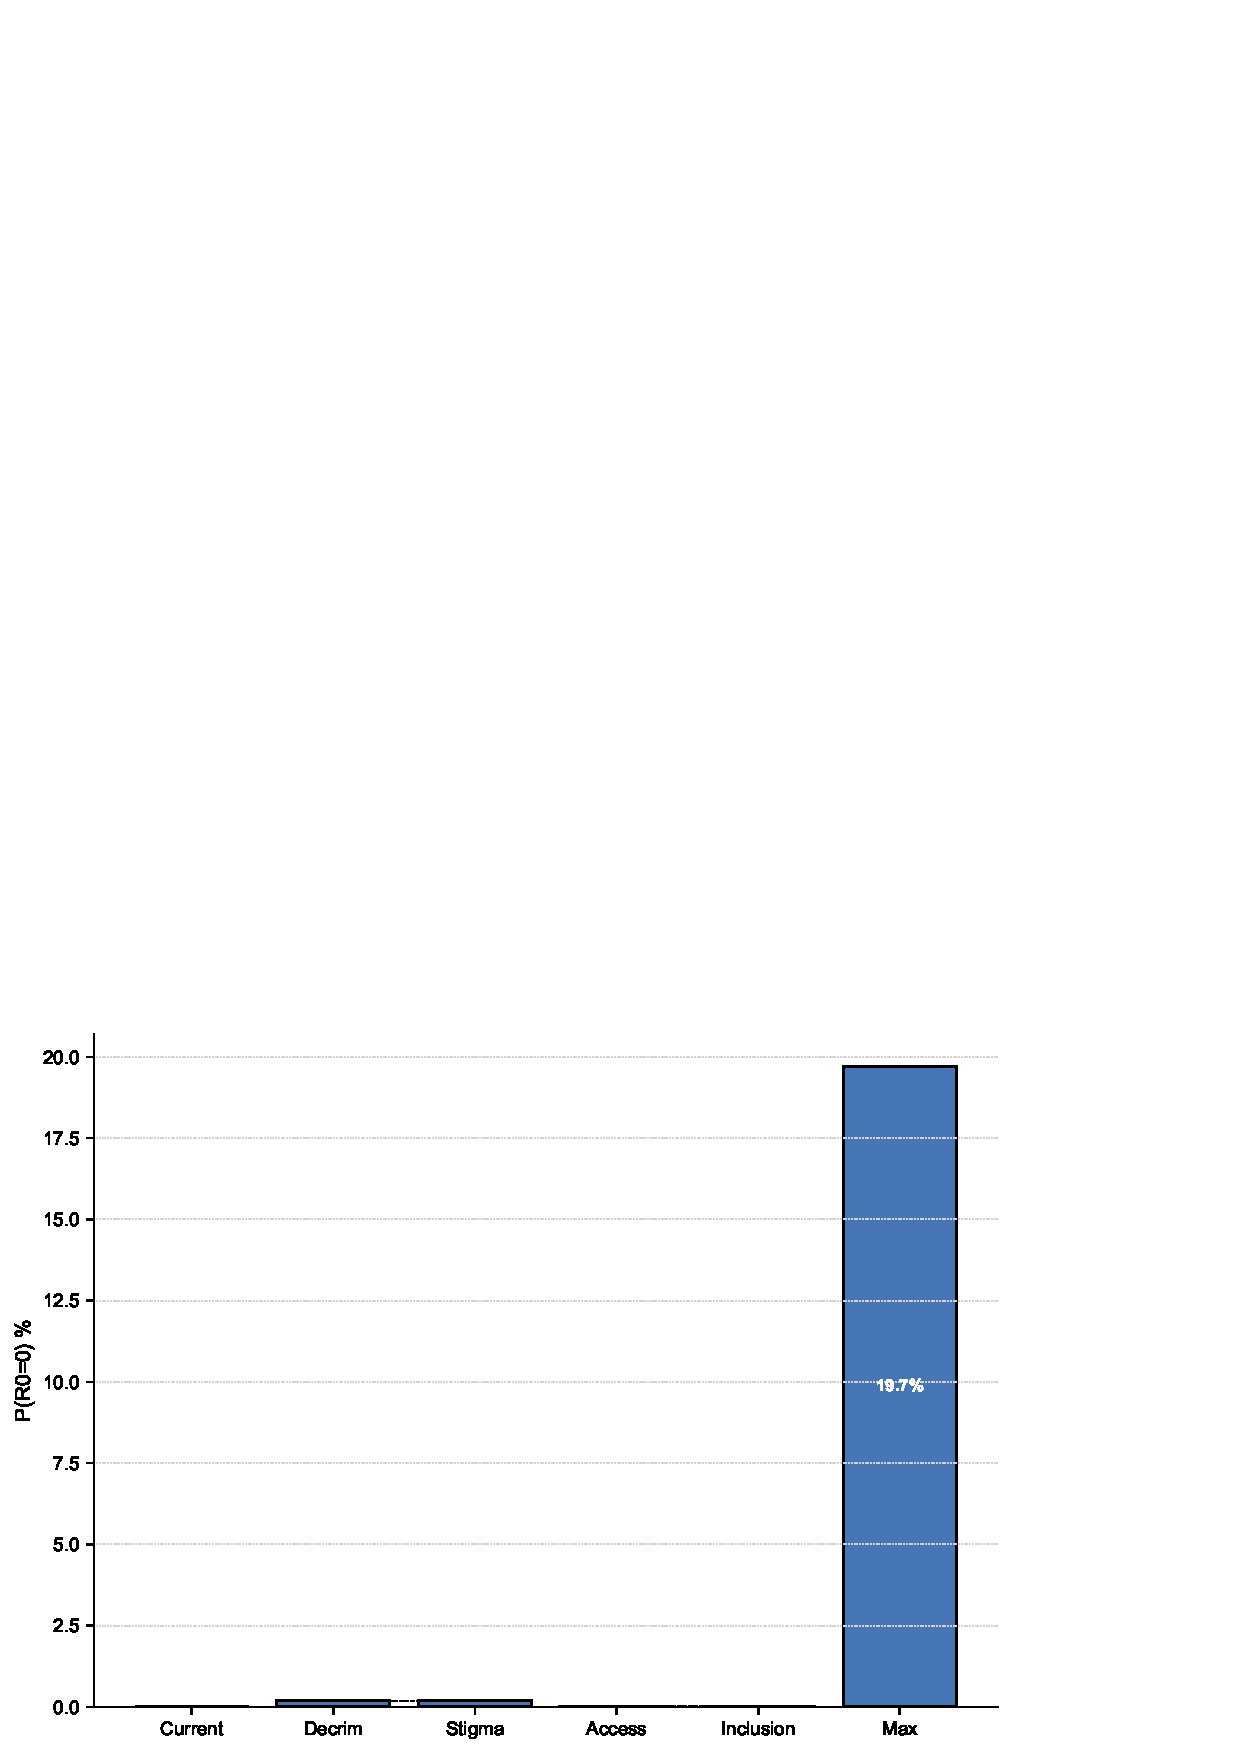
\includegraphics[width=\textwidth]{FigS7_BarrierRemoval.png}
\caption*{Figure S7}
\end{figure}

\begin{figure}[H]
\centering
\includegraphics[width=\textwidth]{FigS8_StepImportance.png}
\caption*{Figure S8}
\end{figure}

\section*{Supplementary Figure Legends}

\textbf{Figure S1–S8. Supplementary analyses supporting cascade failure, barrier dominance, and outbreak inevitability among PWID.}

\textbf{Figure S1. Methamphetamine prevalence trajectories used in stochastic avoidance modeling.}
Projected regional methamphetamine prevalence trajectories among people who inject drugs (PWID) over a 10-year horizon, stratified by U.S. region. Trajectories were parameterized from national surveillance and cohort data demonstrating increasing stimulant injection and opioid–methamphetamine co-use.\cite{golden_outbreak_2019, glick_meth_2018, walters_portland_2022, van_handel_vulnerability_2016, bonacci_kanawha_2023, mcclung_cabell_2021, plankey_meth_2007}

\textbf{Figure S2. Stochastic avoidance failure and outbreak probability over time.}
Cumulative probability of a major HIV outbreak among PWID under current policy conditions, estimated using Monte Carlo simulation incorporating network density evolution, methamphetamine prevalence, housing instability, and incarceration rates.

\textbf{Figure S3. Tornado diagram of parameter sensitivity for 5-year outbreak probability.}
One-way sensitivity analysis showing the relative influence of model parameters on predicted outbreak probability at 5 years.

\textbf{Figure S4. Policy scenario comparison for achieving sustained protection (R$_0$ = 0).}
Comparison of eight policy scenarios illustrating the probability of achieving sustained HIV protection among PWID over 5 years.

\textbf{Figure S5. Cascade uncertainty and probabilistic completion distribution.}
Distribution of prevention cascade completion probabilities across probabilistic sensitivity analyses.

\textbf{Figure S6. Distribution of R$_0$ = 0 outcomes under Monte Carlo simulation.}
Histogram of achieved sustained protection outcomes across 100,000 simulated PWID under current policy conditions.

\textbf{Figure S7. Barrier removal analysis showing incremental gains in prevention probability.}
Sequential removal of individual barrier classes illustrating their incremental contribution to prevention probability.

\textbf{Figure S8. Relative importance of cascade steps in determining prevention failure.}
Step-importance analysis quantifying the proportion of total cascade failure attributable to each prevention stage.

\bibliographystyle{elsarticle-num}
\bibliography{unified_lancet_hiv_2025_acd}



\end{document}